% move all configuration stuff into one file so we can focus on the content
\documentclass[aspectratio=169,hyperref={pdfpagelabels=false,colorlinks=true,linkcolor=white,urlcolor=lightblue},xcolor={table},t]{beamer}

%%%%%%%%%%%%%%%%%%%%%%%%%%%%%%%%%%%%%%%%%%%%%%%%%%%%%%%%%%%%%%%%%%%%%%%%%%%%%%%%%%
%%%%%%%%%%%%%%%%%%%%%%%%%%%%%%%%%%%%%%%%%%%%%%%%%%%%%%%%%%%%%%%%%%%%%%%%%%%%%%%%%%
% packages
\usepackage{pict2e}
\usepackage{epic}
\usepackage{amsmath,amsfonts,amssymb}
\usepackage{units}
\usepackage{fancybox}
\usepackage[absolute,overlay]{textpos} 
%\usepackage[table]{xcolor}
\usepackage{animate}
\usepackage{gensymb}
%\usepackage{graphicx}
%\usepackage{longtable}
\usepackage{multirow}
\usepackage{silence}
\usepackage{tikz}
\usepackage[backend=bibtex,style=ieee]{biblatex}
\AtEveryCitekey{\iffootnote{\tiny}{}}
%\addbibresource{include/references}



% fontsize
\let\Tiny=\tiny

%%%%%%%%%%%%%%%%%%%%%%%%%%%%%%%%%%%%%%%%%%%%%%%%%%%%%%%%%%%%%%%%%%%%%%%%%%%%%%%%%%
%%%%%%%%%%%%%%%%%%%%%%%%%%%%%%%%%%%%%%%%%%%%%%%%%%%%%%%%%%%%%%%%%%%%%%%%%%%%%%%%%%
% warnings
\pdfsuppresswarningpagegroup=1
\WarningFilter{biblatex}{Patching footnotes failed}
\WarningFilter{latexfont}{Font shape}
\WarningFilter{latexfont}{Some font shapes}
\WarningFilter{gensymb}{Not defining}


%%%%%%%%%%%%%%%%%%%%%%%%%%%%%%%%%%%%%%%%%%%%%%%%%%%%%%%%%%%%%%%%%%%%%%%%%%%%%%%%%%
%%%%%%%%%%%%%%%%%%%%%%%%%%%%%%%%%%%%%%%%%%%%%%%%%%%%%%%%%%%%%%%%%%%%%%%%%%%%%%%%%%
% theme & layout
\usetheme{Frankfurt}
\useinnertheme{rectangles}


%%%%%%%%%%%%%%%%%%%%%%%%%%%%%%%%%%%%%%%%%%%%%%%%%%%%%%%%%%%%%%%%%%%%%%%%%%%%%%%%%%
\setbeamertemplate{frametitle}[default][colsep=-4bp,rounded=false,shadow=false]
\setbeamertemplate{frametitle}
{%
    \nointerlineskip%
    %\vskip-0.5ex
    \begin{beamercolorbox}[wd=\paperwidth,ht=3.5ex,dp=0.6ex]{frametitle}
        \hspace*{1.3ex}\insertframetitle%
        
        \hspace*{1.3ex}\small\insertframesubtitle%
    \end{beamercolorbox}%
    \begin{textblock*}{100mm}(13.75cm,1cm)
        
\includegraphics[height=.4cm,keepaspectratio]{../shared/Logo_GTCMT_white}
    \end{textblock*}
}


%%%%%%%%%%%%%%%%%%%%%%%%%%%%%%%%%%%%%%%%%%%%%%%%%%%%%%%%%%%%%%%%%%%%%%%%%%%%%%%%%%
\setbeamertemplate{title page}[default][colsep=-4bp,rounded=false,shadow=false]
\setbeamertemplate{title page}
{
    %\begin{textblock*}{100mm}(15cm,.51cm)
            %\href{https://github.com/alexanderlerch/ACA-Slides/blob/2nd_edition/\jobname.pdf}{\includegraphics[height=.5cm,keepaspectratio]{graph/Logo_github}}\hspace*{2ex}
    %\end{textblock*}
    %\begin{textblock*}{100mm}(15cm,1.3cm)
            %\href{\IEEELink}{\includegraphics[height=.5cm,keepaspectratio]{graph/icon/book}}\hspace*{2ex}
    %\end{textblock*}
    \vskip-10ex
    \begin{beamercolorbox}[wd=\paperwidth,ht=.7\paperheight,dp=0.6ex]{frametitle} %35ex
        %\begin{flushright}
            %\href{http://www.gtcmt.gatech.edu}{
\includegraphics[height=.8cm,keepaspectratio]{graph/Logo_GTCMT_black}}\hspace*{2ex}
        %\end{flushright}
        
        \hspace*{1.8ex}\LARGE\inserttitle%
        
        \vspace*{.5ex}
        
        \hspace*{1.3ex}\small\insertsubtitle%
        
        \vspace*{.5ex}
    \end{beamercolorbox}%
    \nointerlineskip%
    \begin{beamercolorbox}[wd=\paperwidth,ht=.4\paperheight,dp=0.6ex]{page number in head/foot}
        %\vspace*{-.5ex}
        \hspace*{1.7ex}\small\insertauthor%
        
        %\hspace*{1.7ex}\small }%
        
        \vspace*{12ex}
        \vfill
        \begin{flushright}
            \href{http://www.gtcmt.gatech.edu}{
\includegraphics[height=.5cm,keepaspectratio]{../shared/Logo_GTCMT_black}}\hspace*{2ex}
        \end{flushright}
    \end{beamercolorbox}%
}


%%%%%%%%%%%%%%%%%%%%%%%%%%%%%%%%%%%%%%%%%%%%%%%%%%%%%%%%%%%%%%%%%%%%%%%%%%%%%%%%%%
%\makeatother
\setbeamertemplate{footline}
{
  \leavevmode%
  \hbox{%
  \begin{beamercolorbox}[wd=.5\paperwidth,ht=2.25ex,dp=1ex,left,leftskip=1ex]{page number in head/foot}%
    \insertsubtitle
  \end{beamercolorbox}%
  \begin{beamercolorbox}[wd=.5\paperwidth,ht=2.25ex,dp=1ex,right,rightskip=1ex]{page number in head/foot}%
    \hfill
    \insertframenumber{} / \inserttotalframenumber
  \end{beamercolorbox}}%
  \vskip0pt%
}
%\makeatletter


%%%%%%%%%%%%%%%%%%%%%%%%%%%%%%%%%%%%%%%%%%%%%%%%%%%%%%%%%%%%%%%%%%%%%%%%%%%%%%%%%%
\beamertemplatenavigationsymbolsempty
\setbeamertemplate{navigation symbols}{}
\setbeamertemplate{blocks}[default]%[rounded=false,shadow=false]
\setbeamertemplate{itemize item}[square]
\setbeamertemplate{itemize subitem}[circle]
\setbeamertemplate{itemize subsubitem}[triangle]
\setbeamertemplate{enumerate item}[square]
\setbeamertemplate{enumerate subitem}[circle]
\setbeamertemplate{enumerate subsubitem}[circle]


%%%%%%%%%%%%%%%%%%%%%%%%%%%%%%%%%%%%%%%%%%%%%%%%%%%%%%%%%%%%%%%%%%%%%%%%%%%%%%%%%%
% colors
\setbeamercolor{structure}{fg=darkgray}
\setbeamercovered{transparent} %invisible
\setbeamercolor{bibliography entry author}{fg=black}
\setbeamercolor*{bibliography entry title}{fg=black}
\setbeamercolor*{bibliography entry note}{fg=black}
\setbeamercolor{frametitle}{fg=black}
\setbeamercolor{title}{fg=white}
\setbeamercolor{subtitle}{fg=white}
\setbeamercolor{frametitle}{fg=white}
\setbeamercolor{framesubtitle}{fg=white}
\setbeamercolor{mini frame}{fg=white, bg=black}
\setbeamercolor{section in head/foot}{fg=white, bg=darkgray}
\setbeamercolor{page number in head/foot}{fg=black, bg=gtgold}
\setbeamercolor{item projected}{fg=white, bg=black}

%---------------------------------------------------------------------------------

%%%%%%%%%%%%%%%%%%%%%%%%%%%%%%%%%%%%%%%%%%%%%%%%%%%%%%%%%%%%%%%%%%%%%%%%%%%%%%%%%%
%%%%%%%%%%%%%%%%%%%%%%%%%%%%%%%%%%%%%%%%%%%%%%%%%%%%%%%%%%%%%%%%%%%%%%%%%%%%%%%%%%
% title information
\title[]{MUSI6202: Digital Signal Processing for Music}   
\author[alexander lerch]{alexander lerch} 
%\institute{~}
%\date[Alexander Lerch]{}
%\titlegraphic{\vspace{-16mm}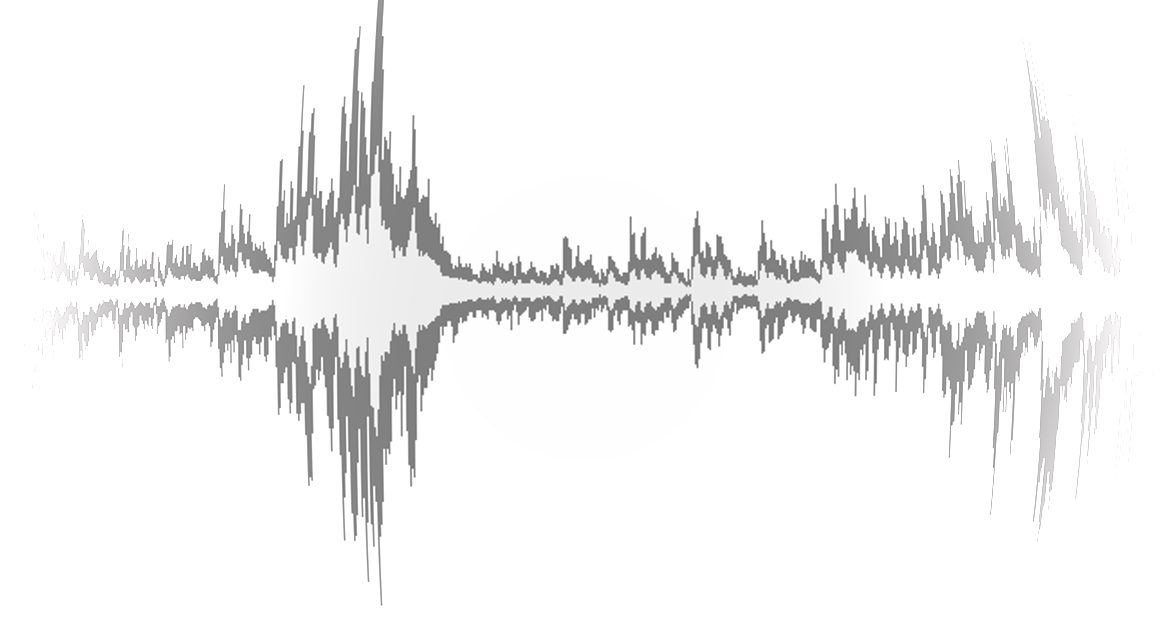
\includegraphics[width=\textwidth,height=3cm]{title}}

%%%%%%%%%%%%%%%%%%%%%%%%%%%%%%%%%%%%%%%%%%%%%%%%%%%%%%%%%%%%%%%%%%%%%%%%%%%%%%%%%%
%%%%%%%%%%%%%%%%%%%%%%%%%%%%%%%%%%%%%%%%%%%%%%%%%%%%%%%%%%%%%%%%%%%%%%%%%%%%%%%%%%
% colors
\definecolor{gtgold}{rgb}{.914, .664, 0} %0e7eed {rgb}{0.88,0.66,1,0.06} [234, 170, 0]/256 %96caff
\definecolor{darkgray}{rgb}{.15, .15, .15}
\definecolor{lightblue}{HTML}{0e7eed}
\definecolor{highlight}{rgb}{0, 0, 1} %_less!40

%%%%%%%%%%%%%%%%%%%%%%%%%%%%%%%%%%%%%%%%%%%%%%%%%%%%%%%%%%%%%%%%%%%%%%%%%%%%%%%%%%
%%%%%%%%%%%%%%%%%%%%%%%%%%%%%%%%%%%%%%%%%%%%%%%%%%%%%%%%%%%%%%%%%%%%%%%%%%%%%%%%%%
% relative paths
\graphicspath{{../graph/}}


%%%%%%%%%%%%%%%%%%%%%%%%%%%%%%%%%%%%%%%%%%%%%%%%%%%%%%%%%%%%%%%%%%%%%%%%%%%%%%%%%%
%%%%%%%%%%%%%%%%%%%%%%%%%%%%%%%%%%%%%%%%%%%%%%%%%%%%%%%%%%%%%%%%%%%%%%%%%%%%%%%%%%
% units
\setlength{\unitlength}{1mm}

%%%%%%%%%%%%%%%%%%%%%%%%%%%%%%%%%%%%%%%%%%%%%%%%%%%%%%%%%%%%%%%%%%%%%%%%%%%%%%%%%%
%%%%%%%%%%%%%%%%%%%%%%%%%%%%%%%%%%%%%%%%%%%%%%%%%%%%%%%%%%%%%%%%%%%%%%%%%%%%%%%%%%
% math
\DeclareMathOperator*{\argmax}{argmax}
\DeclareMathOperator*{\argmin}{argmin}
\DeclareMathOperator*{\atan}{atan}
\DeclareMathOperator*{\arcsinh}{arcsinh}
\DeclareMathOperator*{\sign}{sign}
\DeclareMathOperator*{\tcdf}{tcdf}
\DeclareMathOperator*{\si}{sinc}
\DeclareMathOperator*{\princarg}{princarg}
\DeclareMathOperator*{\arccosh}{arccosh}
\DeclareMathOperator*{\hwr}{HWR}
\DeclareMathOperator*{\flip}{flip}
\DeclareMathOperator*{\sinc}{sinc}
\DeclareMathOperator*{\floor}{floor}
\newcommand{\e}{{e}}
\newcommand{\jom}{\mathrm{j}\omega}
\newcommand{\jOm}{\mathrm{j}\Omega}
\newcommand   {\mat}[1]    		{\boldsymbol{\uppercase{#1}}}		%bold
\renewcommand {\vec}[1]    		{\boldsymbol{\lowercase{#1}}}		%bold

%%%%%%%%%%%%%%%%%%%%%%%%%%%%%%%%%%%%%%%%%%%%%%%%%%%%%%%%%%%%%%%%%%%%%%%%%%%%%%%%%%
%%%%%%%%%%%%%%%%%%%%%%%%%%%%%%%%%%%%%%%%%%%%%%%%%%%%%%%%%%%%%%%%%%%%%%%%%%%%%%%%%%
% media9
\newcommand{\includeaudio}[1]{
\href{run:audio/#1.mp3}{
\includegraphics[width=5mm, height=5mm]{graph/SpeakerIcon}}}

\newcommand{\includeanimation}[4]{{\begin{center}
                        \animategraphics[autoplay,loop,scale=.7]{#4}{animation/#1-}{#2}{#3}        
                        \end{center}
                        \addreference{matlab source: \href{https://github.com/alexanderlerch/ACA-Plots/blob/master/matlab/animate#1.m}{matlab/animate#1.m}}}
                        \inserticon{video}}
                        
%%%%%%%%%%%%%%%%%%%%%%%%%%%%%%%%%%%%%%%%%%%%%%%%%%%%%%%%%%%%%%%%%%%%%%%%%%%%%%%%%%
%%%%%%%%%%%%%%%%%%%%%%%%%%%%%%%%%%%%%%%%%%%%%%%%%%%%%%%%%%%%%%%%%%%%%%%%%%%%%%%%%%
% other commands
\newcommand{\question}[1]{%\vspace{-4mm}
                          \setbeamercovered{invisible}
                          \begin{columns}[T]
                            \column{.9\textwidth}
                                \textbf{#1}
                            \column{.1\textwidth}
                                \vspace{-8mm}
                                \begin{flushright}
                                     
\includegraphics[width=.9\columnwidth]{graph/question_mark}
                                \end{flushright}
                                \vspace{6mm}
                          \end{columns}\pause\vspace{-12mm}}

\newcommand{\toremember}[1]{
                        \inserticon{lightbulb}
                        }

\newcommand{\matlabexercise}[1]{%\vspace{-4mm}
                          \setbeamercovered{invisible}
                          \begin{columns}[T]
                            \column{.8\textwidth}
                                \textbf{matlab exercise}: #1
                            \column{.2\textwidth}
                                \begin{flushright}
                                     \includegraphics[scale=.5]{graph/logo_matlab}
                                \end{flushright}
                                %\vspace{6mm}
                          \end{columns}}

\newcommand{\addreference}[1]{  
                  
                    \begin{textblock*}{\baselineskip }(.98\paperwidth,.5\textheight) %(1.15\textwidth,.4\textheight)
                         \begin{minipage}[b][.5\paperheight][b]{1cm}%
                            \vfill%
                             \rotatebox{90}{\tiny {#1}}
                        \end{minipage}
                   \end{textblock*}
                    }
                    
\newcommand{\figwithmatlab}[1]{
                    \begin{figure}
                        \centering
                        \includegraphics[scale=.7]{#1}
                        %\label{fig:#1}
                    \end{figure}
                    
                    \addreference{matlab source: \href{https://github.com/alexanderlerch/MUSI-6202/blob/main/matlab/plot#1.m}{plot#1.m}}}
\newcommand{\figwithref}[2]{
                    \begin{figure}
                        \centering
                        \includegraphics[scale=.7]{#1}
                        \label{fig:#1}
                    \end{figure}
                    
                    \addreference{#2}}  
                                    
\newcommand{\inserticon}[1]{
                    \begin{textblock*}{100mm}(14.5cm,7.5cm)
                        \includegraphics[height=.8cm,keepaspectratio]{graph/#1}
                    \end{textblock*}}            

%%%%%%%%%%%%%%%%%%%%%%%%%%%%%%%%%%%%%%%%%%%%%%%%%%%%%%%%%%%%%%%%%%%%%%%%%%%%%%%%%%
%%%%%%%%%%%%%%%%%%%%%%%%%%%%%%%%%%%%%%%%%%%%%%%%%%%%%%%%%%%%%%%%%%%%%%%%%%%%%%%%%%
% counters
\newcounter{i}
\newcounter{j}
\newcounter{iXOffset}
\newcounter{iYOffset}
\newcounter{iXBlockSize}
\newcounter{iYBlockSize}
\newcounter{iYBlockSizeDiv2}
\newcounter{iXBlockSizeDiv2}
\newcounter{iDistance}

\newcommand{\IEEELink}{https://ieeexplore.ieee.org/servlet/opac?bknumber=9965970}

\addbibresource{../shared/references}



\subtitle{Part 6: LTI Systems \& Convolution}

%%%%%%%%%%%%%%%%%%%%%%%%%%%%%%%%%%%%%%%%%%%%%%%%%%%%%%%%%%%%%%%%%%%%%%%%%%%%
\begin{document}
    % generate title page
	\title[]{Digital Signal Processing for Music}   
\author[alexander lerch]{alexander lerch} 
%\institute{~}
%\date[Alexander Lerch]{}
\titlegraphic{\vspace{-16mm}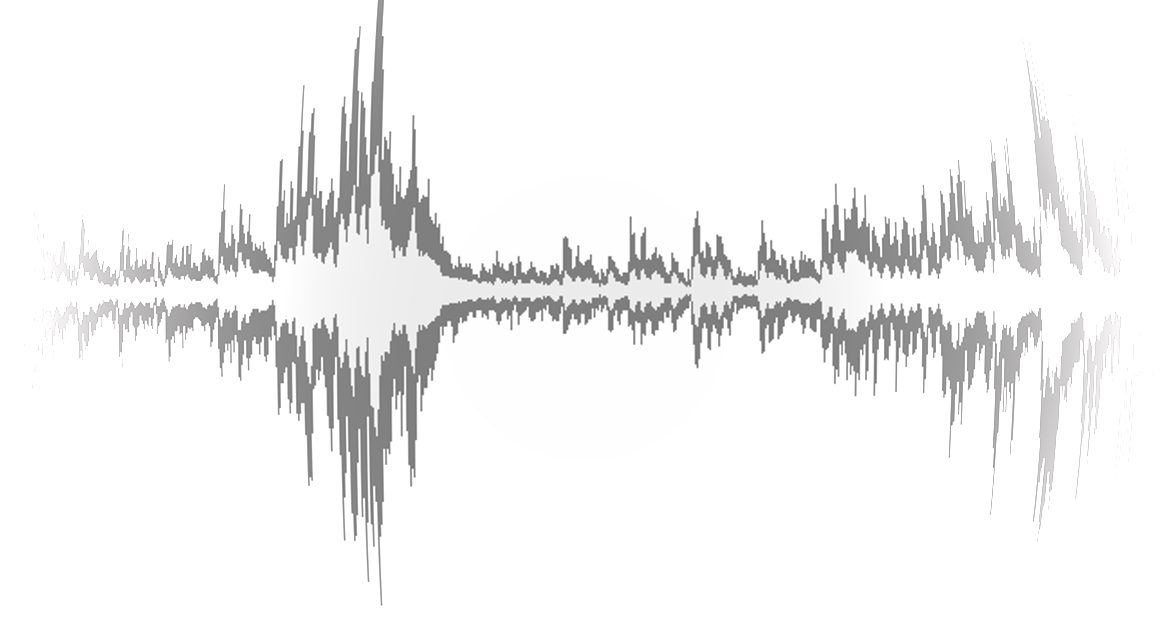
\includegraphics[width=\textwidth,height=3cm]{title}}


\begin{frame}
    \titlepage
    %\vspace{-5mm}
    \begin{flushright}
        \href{http://www.gtcmt.gatech.edu}{
\includegraphics[height=.8cm,keepaspectratio]{../shared/Logo_GTCMT_black}}
    \end{flushright}
\end{frame}


    \section[intro]{introduction}
        \begin{frame}{lecture content}{overview}
            \begin{enumerate}
                \item   LTI systems and their properties
                \smallskip
                \item   convolution
            \end{enumerate}
        \end{frame}

        \begin{frame}{systems}{introduction}
            a system:
            \begin{itemize}
                \item   any process producing an output signal in response to an input signal
            \end{itemize}
		    \begin{figure}
				\centering
		        \begin{picture}(80,35)
		            %boxes
		            %\put(0,30){\ovalbox{\footnotesize{\parbox{20mm}{\vspace{2mm}\centering{Composer}\vspace{2mm}}}}}
		            \put(30,30){\ovalbox{\footnotesize{\parbox{20mm}{\vspace{2.3mm}\centering{System}\vspace{2.3mm}}}}}
		            %\put(60,30){\ovalbox{\footnotesize{\parbox{20mm}{\vspace{2mm}\centering{Recipient}\vspace{2mm}}}}}
		
		            % horizontal
		            \put(22.4,30.6){\vector(1,0){7.8}}
		            \put(52.4,30.6){\vector(1,0){7.8}}
		            \put(15,30){\text{$x(t)$}}
		            \put(60,30){\text{$y(t)$}}
		        \end{picture}
		    \end{figure}
            \vspace{-25mm}
            \question{name examples for systems in signal processing/the real world}
            
            \begin{itemize}
                \item   filters, effects
                \item   vocal tract
                \item   room
                \item   (audio) cable
                \item   \ldots
            \end{itemize}
        \end{frame}
    \section[LTI]{Linear Time-Invariant systems}
        \begin{frame}{systems}{linearity and non-linearity}
            \begin{columns}
            \column{.7\linewidth}
            \begin{itemize}
                \item   examples for mostly linear systems:
                    \begin{itemize}
                        \item   room
                        \item   eq
                    \end{itemize}
                \bigskip
                \item   examples for non-linear systems:
                    \begin{itemize}
                        \item   diode
                        \item   vacuum tube
                    \end{itemize}
            \end{itemize}
            \column{.3\linewidth}
            \begin{figure}%
                \includegraphics[scale=.75]{graph/linearnonlinear}%
            \end{figure}
            \end{columns}

            \addreference{\url{http://www.sfu.ca/sonic-studio/handbook/Linear.html}}
        \end{frame}

        \begin{frame}{systems}{linearity}
            \toremember{linearity is defined by two properties}
            
            \begin{enumerate}
                \item   \textbf{homogeneity}:
                    \[f(ax) = a f(x)\]
                \bigskip
                \item   \textbf{superposition} (additivity):
                \[f(x+y) = f(x) + f(y)\]
            \end{enumerate}
        \end{frame}
        \begin{frame}{systems}{time invariance}
            \toremember{time invariance}
            
            \begin{itemize}
                \item   does not change with time:
                    \[f\left(x(t-\tau)\right) = f(x)(t-\tau)\]
            \end{itemize}
            \pause
            \bigskip
            \begin{block}{LTI: Linear Time-invariant Systems}
                are a great simplification for many real-world systems we would like to model --- circuits, spring-mass-damper systems, etc.
            \end{block}
        \end{frame}
        \begin{frame}{systems}{LTI system example}
            velocity of mass an a table
            \begin{enumerate}
                \item   hammer gives \textit{impulse}
                \item   system \textit{responds} with velocity
                \bigskip
                \item<2->[]   \textbf{linearity}:\\ double force, double velocity, multiple strikes add up
                \smallskip
                \item<2->[]   \textbf{time invariance}:\\ system reacts the same whether I do it now or tomorrow
            \end{enumerate}
        \end{frame}
        \begin{frame}{systems}{other system characteristics}
            \begin{itemize}
                \item   \textbf{causality}:\\ output depends only on past and present input
                \bigskip
                \item   \textbf{BIBO stability}:\\ output is bounded for bounded input
            \end{itemize}
        \end{frame}
    \section{convolution}
        \begin{frame}{convolution}{introduction}
            \question{we know how a system reacts to an impulse, but what of a more complex input signal}

            \begin{itemize}
                \item<2-> assume that the signal is constructed from many densely packed impulses
                \item<2->[$\Rightarrow$] output is superposition of all individual responses
            \end{itemize}
            \pause
            \bigskip
            \textbf{convolution}
            \begin{equation*}
                y(t) = (x \ast h)(t) := \int\limits_{-\infty}^{\infty}x(\tau)h(t-\tau)d\tau
            \end{equation*}
        \end{frame}
\begin{frame}{convolution}{animation}
            \vspace{-5mm}
            \includeanimation{Convolution}{000}{600}{10}
\end{frame}
    
\begin{frame}\frametitle{convolution}\framesubtitle{exercise --- convolution by hand}
    compute the convolution of the following two signals $y(n) = x(n) * v(n)$
    \figwithmatlab{ConvolutionByHand}
    
    \vspace{-4mm}
    \begin{columns}
    \column{.4\linewidth}
        steps:
        \begin{enumerate}
            \item   flip one signal
            \item   multiply the two signals
            \item   integrate the result
            \item   shift
            \item   go to 2.
        \end{enumerate}
    \column{.6\linewidth}
        \only<2>{
        \begin{figure}%
            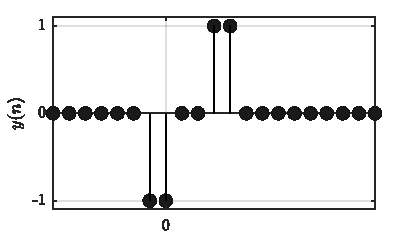
\includegraphics[scale=.7]{ConvolutionByHand-Solution}
        \end{figure}
        }
    \end{columns}
\end{frame}
    
\section[conv. prop.]{convolution properties}
\begin{frame}\frametitle{convolution}\framesubtitle{identity and impulse response}
    \begin{eqnarray*}
        x(t) &=& \delta(t)\ast x(t) \\
        h(t) &=& \delta(t)\ast h(t) 
    \end{eqnarray*}

    \bigskip
    \begin{itemize}
        \item<2->   describes the response of a system to an impulse as a function of time
        \smallskip
        \item<3->   as an impulse includes all frequencies, the resulting IR defines the response for all frequencies
        \smallskip
        \item<4->   the convolution of $\delta(t)$ with a signal/impulse response results in that impulse response
    \end{itemize}
\end{frame}
    
	\begin{frame}\frametitle{convolution}\framesubtitle{properties}
		\begin{equation*}
			y(t) = x(t) \ast h(t) = \int\limits_{-\infty}^{\infty}{h(\tau)\cdot x(t-\tau)} d\tau
		\end{equation*}
		\begin{itemize}
			\item	\textbf{commutativity}
				\begin{equation*}
					h(t) \ast x(t)	= x(t) \ast h(t)
				\end{equation*}
			\pause
			\item	\textbf{associativity}
				\begin{equation*}
					\big(g(t) \ast h(t)\big) \ast x(t) = g(t) \ast \big(h(t) \ast x(t)\big)
				\end{equation*}
			\pause
			\item	\textbf{distributivity}
				\begin{equation*}
					g(t) \ast \big(h(t) + x(t)\big) = \big(g(t) \ast h(t)\big) + \big(g(t) \ast x(t)\big)
				\end{equation*}
		\end{itemize}
\end{frame}

\section[deriv]{convolution property derivation}

\begin{frame}\frametitle{convolution}\framesubtitle{derivation: commutativity}
\begin{footnotesize}
		\begin{equation*}
			h(t) \ast x(t)	= x(t) \ast h(t) 
		\end{equation*}
		
        \bigskip
        substituting $\tau'=t-\tau$:
		\begin{eqnarray*}
			x(t) \ast h(t)
					&=& \int\limits_{-\infty}^{\infty}{h(\tau)\cdot x(t-\tau)} d\tau\nonumber\\
                    \pause&=& \int\limits_{-\infty}^{\infty}{h(t-\tau')\cdot x(\tau')}d(t-\tau') \nonumber\\
					\pause&=& \int\limits_{-\infty}^{\infty}{x(\tau')\cdot h(t-\tau')}d\tau' 
		\end{eqnarray*}
\end{footnotesize}
\end{frame}	

\begin{frame}\frametitle{convolution}\framesubtitle{derivation: associativity}
\vspace{-6mm}
\begin{footnotesize}
		\begin{equation*}
			\big(g(t) \ast h(t)\big) \ast x(t) = g(t) \ast \big(h(t) \ast x(t)\big)
		\end{equation*}
		changing the order of sums and shifting the operands as shown below:
		\begin{eqnarray*}
			\big(g(t) \ast h(t)\big) \ast x(t)	&=& \int\limits_{\tau=-\infty}^{\infty}{\big(g(\tau) \ast h(\tau)\big)\cdot x(t-\tau)}d\tau\nonumber\\
%												&=& \int\limits_{\tau=-\infty}^{\infty}{\left(\sum\limits_{\xi=-\infty}^{\infty}{g(\xi)\cdot h(\tau-\xi)}\cdot x(t-\tau)\right)}\nonumber\\
												\pause&=& \int\limits_{-\infty}^{\infty}{\int\limits_{-\infty}^{\infty}{g(\xi)\cdot h(\tau-\xi)}\cdot x(t-\tau)}d\tau d\xi\nonumber\\
												\pause&=& \int\limits_{-\infty}^{\infty}{g(\xi)\cdot \int\limits_{-\infty}^{\infty}{h(\tau-\xi)}\cdot x(t-\tau)}d\tau d\xi\nonumber\\
												\pause&=& \int\limits_{-\infty}^{\infty}{g(\xi)\cdot \int\limits_{-\infty}^{\infty}{h(\tau')}\cdot x(t-\xi-\tau')d\tau' d\xi}\nonumber\\
												\pause&=& \int\limits_{-\infty}^{\infty}{g(\xi)\cdot  \big(h(t-\xi) \ast x(t-\xi)\big)} d\xi\nonumber\\
												\pause&=& g(t) \ast \big(h(t) \ast x(t)\big) 
		\end{eqnarray*}
\end{footnotesize}
\end{frame}	

\begin{frame}\frametitle{convolution}\framesubtitle{derivation: distributivity}
\begin{footnotesize}
		\begin{equation*}
			g(t) \ast \big(h(t) + x(t)\big) = g(t) \ast h(t) + g(t) \ast x(t) 
		\end{equation*}
		\begin{eqnarray*}
			g(t) \ast \big(h(t) + x(t)\big) &=& \int\limits_{-\infty}^{\infty}{g(\tau) \cdot\big(h(t-\tau) + x(t-\tau)\big)}d\tau\nonumber\\
									\pause&=& \int\limits_{-\infty}^{\infty}{g(\tau) \cdot h(t-\tau) + g(\tau) \cdot x(t-\tau)}d\tau\nonumber\\
									\pause&=& \int\limits_{-\infty}^{\infty}{g(\tau) \cdot h(t-\tau)}d\tau + \int\limits_{-\infty}^{\infty}{g(\tau) \cdot x(t-\tau)}d\tau\nonumber\\
									\pause&=& g(t) \ast h(t) + g(t) \ast x(t) 
		\end{eqnarray*}
\end{footnotesize}
\end{frame}	

    \section[summary]{summary}
        \begin{frame}{systems}{summary}
            \vspace{-3mm}
            \begin{itemize}
                \item   \textbf{LTI system}: approximation of many real-world systems
                    \begin{itemize}
                    \item<2-> properties:
                        \begin{itemize}
                            \item   linearity 1: homogeneity (scaling)
                            \item   linearity 2: superposition (additivity)
                            \item   time invariance (system doesn't change)
                            \item<3->   causality (no future input)
                            \item<3->   BIBO --- bounded input bounded output
                        \end{itemize}
                    \end{itemize}
                \bigskip
                \item<4-> \textbf{impulse response} is a complete description of an LTI system
                \bigskip
                \item<5-> \textbf{convolution}: describes process of generating output of LTI system from input
                    \begin{itemize}
                    \item<6-> properties:
                        \begin{itemize}
                            \item   commutative
                            \item   associative
                            \item   distributive
                        \end{itemize}
                    \end{itemize}
            \end{itemize}
        \end{frame}

    
\end{document}

